\documentclass{article}
\usepackage[doublespacing]{setspace}
\usepackage[utf8]{inputenc}
\usepackage{hyperref}
\usepackage{enumitem}
\usepackage[english]{babel}
\usepackage{lineno}
\usepackage[round]{natbib}
\usepackage{graphicx}
\usepackage{float}
\usepackage{amsmath}
\usepackage{amsthm}
\usepackage{amssymb}
\usepackage{bm}
\usepackage{subfig}
\usepackage{cleveref}
\usepackage{lipsum}
\usepackage{listings}

\title{Example \LaTeX{} Document with a new title}
\author{Johannes and César}
\date{\today}

\linenumbers
\numberwithin{equation}{section}
\begin{document}

\maketitle

\newpage


\tableofcontents
\listoffigures
\listoftables

\newpage

\section{Introduction}\label{intro}
super and subscript: 10$^2$ 4$_f$ special characters: äáÈß\ss. A nice citation: \cite{hipsey_2019}.

There is a theory which states that if ever anyone discovers exactly what the Universe is for and why it is here, it will
instantly disappear and be replaced by something even more bizarre and inexplicable.
There is another theory which states that this has already happened  \citep{adams1995hitchhiker}.


\begin{figure}[t]
\centering
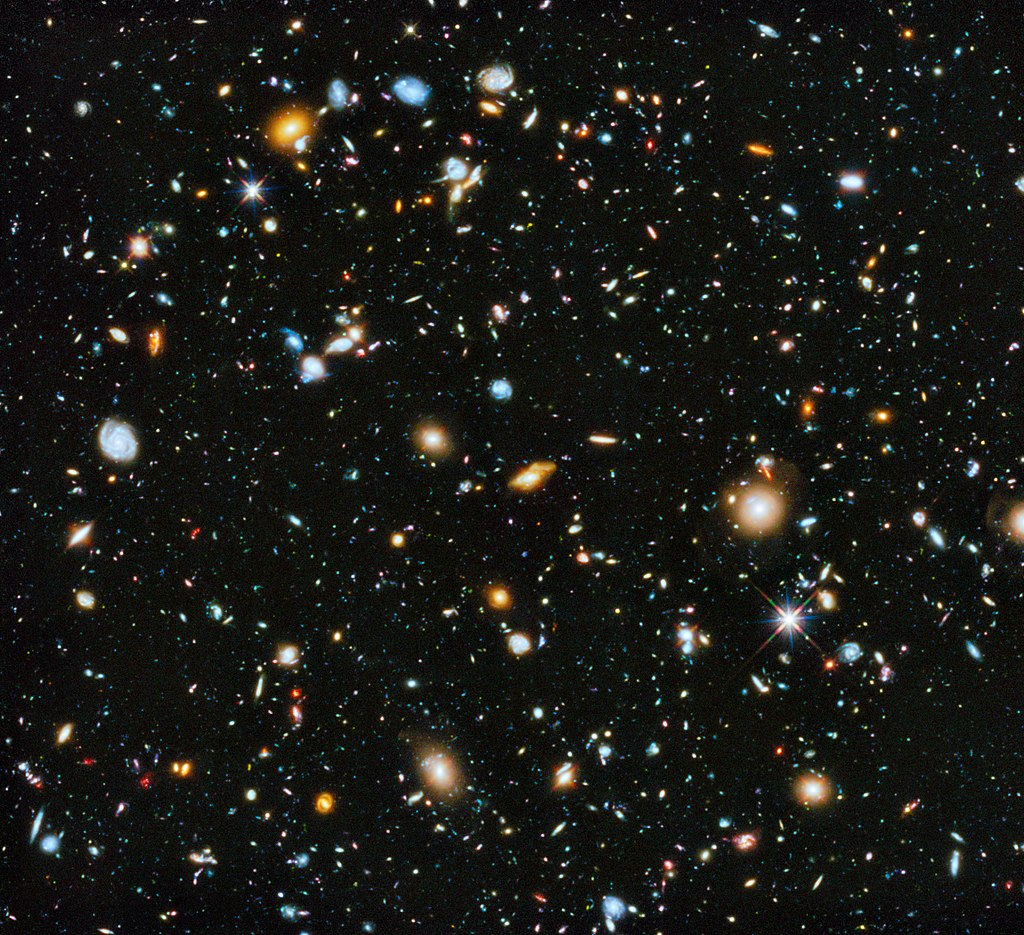
\includegraphics[width=0.5\linewidth]{universe.jpg}
\caption[The Universe]{The universe. Picture from NASA (\url{http://www.nasa.gov/hubble})}
\label{fig:galaxy}
\end{figure}

\section{Bullet points and numbering}

\begin{itemize}
    \item First Item
    \item Second item
    \item Another Item with numbered sub-items
    \begin{enumerate}
        \item Important stuff
        \item More important stuff
    \end{enumerate}
    \item And one last item
\end{itemize}

\section{Equations}

\subsection{Equation environments}
First equation using the equation environment:

\begin{equation}
y = a \cdot x + b
\end{equation}

Second equation using the align environment. This is useful for several equations that need to be aligned. The equations are aligned along the \& sign.

\begin{align}
y_1 &= a_{1,1} \cdot x_1 + a_{1,2} \cdot x_2 + b_1 \\
y_2 &= a_{2,1} \cdot x_1 + a_{2,2} \cdot x_2 + a_{2,3} \cdot x_3 b_2 + b_2 \\
y_3 &= a_{3,1} \cdot x_3 + b_3
\end{align}

\subsection{Equations in text}

A equation in running text $y = \frac{1}{x}$.

\section{Tables}

We can refer to \cref{tab:my_label} using the \texttt{\textbackslash{}cref\{key\}} command.

\begin{table}[b]
    \centering
    \caption[First table]{Caption of the table}
    \label{tab:my_label}
    \begin{tabular}{lll}\hline
        Name & ID & Value\\\hline
         Temp & 1  & 14  \\
         Temp & 2  & 16 \\
         Temp & 3 & 15 \\ \hline
    \end{tabular}
\end{table}

\section{Figures}

\subsection{One simple figure}
The milky way is the galaxy that contains our Solar System (\cref{fig:galaxy}).

\subsection{Multiple sub-figures}


\begin{figure}[t]%
    \centering
    \subfloat[The moon mission]{{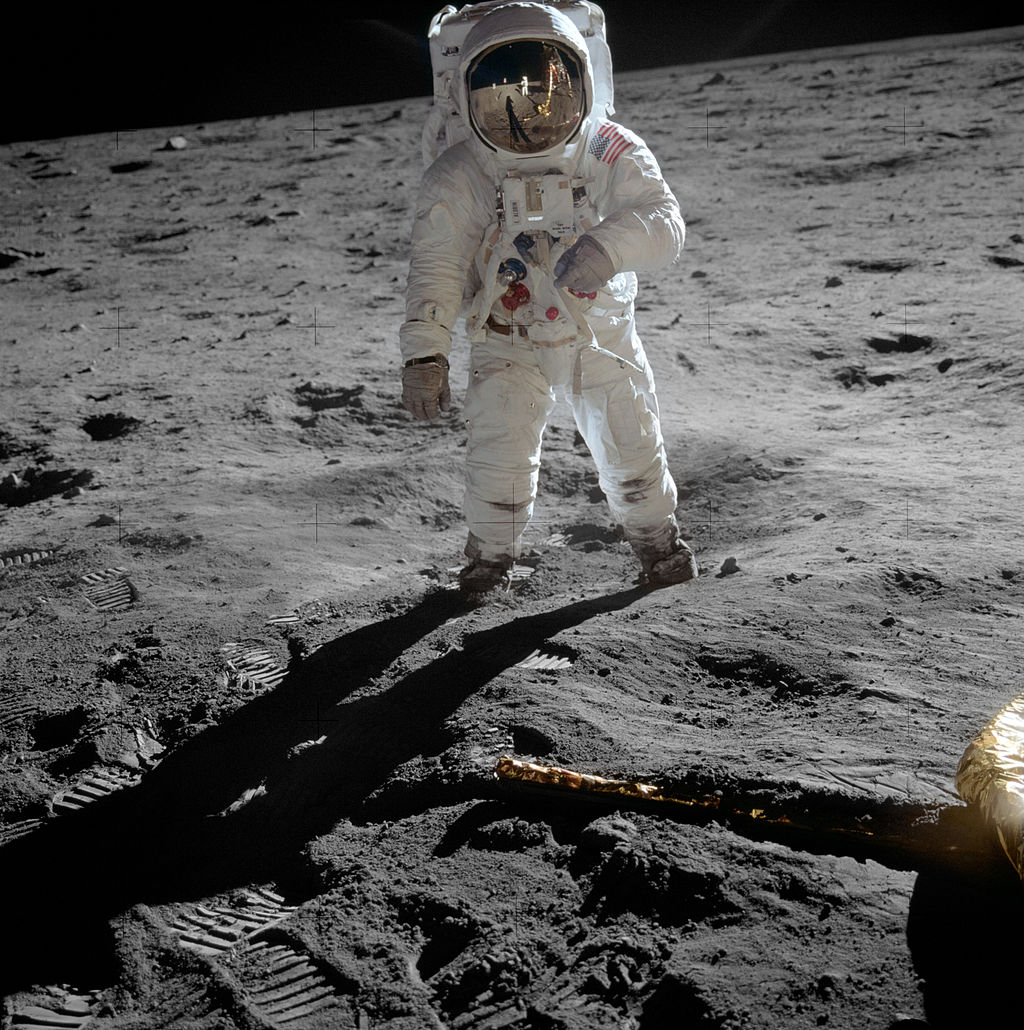
\includegraphics[width=5.5cm]{space-program-post.jpg} }}%
    \qquad
    \subfloat[International space station]{{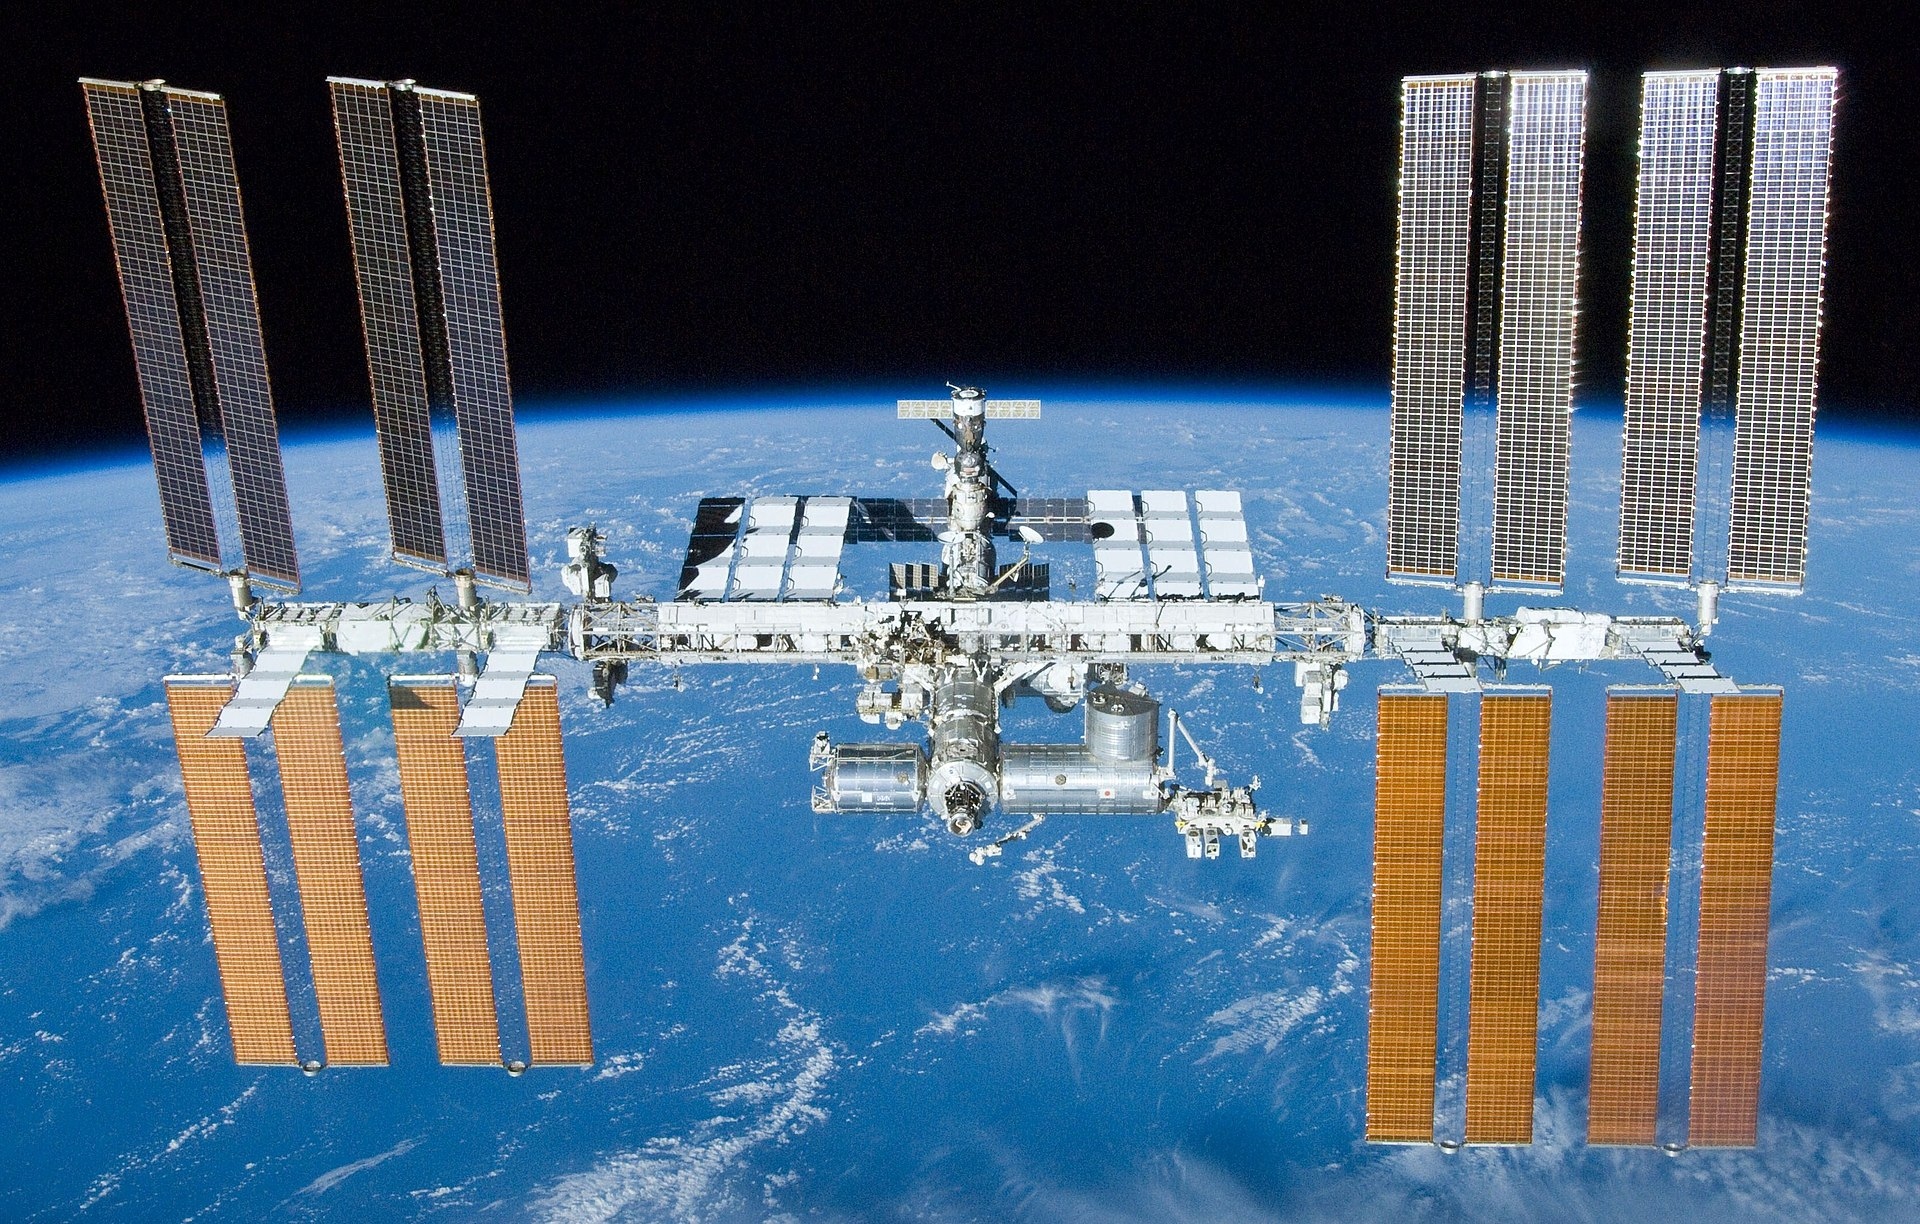
\includegraphics[width=5.5cm]{space-F.jpg} }}%
    \caption{Various space missions. Pictures from NASA.}%
    \label{fig:space}%
\end{figure}



In order to understand and unbox the mysteries of the universe as mentioned in \cref{intro}, scientists have launched various space programs (\cref{fig:space}).

\section{Tasks}

Please try to complete all given tasks. If you already have some experience try the advanced tasks in addition.

\subsection{Basic tasks:}

\begin{enumerate}
	\item Change the author name to your name
	\item Change the title of the document
    \item Include some of your own text
    \item Make some of your text bold and italics
    \item Change the fontsize of some of your text
    \item Include your favorite equation
    \item Include a figure you created
    \item Change the \textit{placement specifier} in a float and see what happens
    \item Change the alignment of one of your figures from centered to the left side
    \item Add your own table
    \item Refer to a (sub)section and the page it is on
    \item Add you own reference and cite them
    \item Try different style of referencing (Hint: use of different variations of command cite)
\end{enumerate}

\subsection{Advanced tasks:}

\begin{itemize}
    \item Change the used font
    \item Change the linespacing
    \item Add linenumbers
    \item Change the way equations are numbered so they start with the number of the section and then start counting by 1 in every section
    \item Change the symbol (point) in an \texttt{itemize} list
	\item Change the document to a two column format
    \item Add a table with customized text alignment in different columns and some combined columns
    \item Change the document from article style to any journal style of choice
    \item create a \LaTeX{} table from your own results using R (or python, or Matlab, or ...): an useful package in R is \textit{xtable} and \texttt{print.xtable()}
    \item Find your own Problem/idea and try to implement it

\end{itemize}


\section{Solutions}\label{sec:solutions}

\subsection{Basic tasks:}

Here is some of my own text. Wow that was really not that hard. \textbf{And} this text has \textit{some} parts in \textbf{bold} and \textit{italics}.

{\large this part is written in \texttt{\textbackslash large}}

{\small this part is written in \texttt{\textbackslash small}}

and now here is my favorite equation:

\begin{equation}
	y = \beta_0 + \sum_{i=1}^{n}\beta_i  x_i +  \bm{\beta_{s}} \bm{s} +
	\sum_{i=1}^{n} \bm{\beta_{i:s}} \bm{s} x_i + \bm{\beta_{r}}  \bm{r} +
	\sum_{i=1}^{n} \bm{\beta_{i:r}} \bm{r} x_i + \bm{r}^\intercal \bm{B_{r:s}} \bm{s},
\end{equation}

this is a figure I created with a placement specifier set to \texttt{h!} and left aligned

\begin{figure}[h!]
	\raggedright
	
\includegraphics[width=0.25\linewidth]{my_image}
	\caption[short text]{long caption text for my figure}
\end{figure}

my own table is this:

	\begin{table}[h!]
	\centering
	\caption{Main morphological features and withdrawal depths of the three investigated reservoirs.}
	\label{tab:reservoirs}
	\tiny
	\begin{tabular}{lllllllll}\hline
		Reservoir    & Depth & Surface   & Volume     & Altitude & Latitude    &
		Longitude  & Withdrawal \\
		&   	 (m)	 &	 ($\cdot 10^6$ m$^2$)     & ($\cdot10^6$ m$^3$)    &  (m asl)   &
		($^\circ$N) & ($^\circ$E) & depths (m asl)\\ \hline
		Eibenstock   &  54          & 4.11        & 86.12  & 543          & 50.53     & 12.60    & 487, 498, 504,  \\
		&&&&&&& 514, 519, 524,\\
		&&&&&&&  529\\
		Lichtenberg  &  39          & 0.93        & 14.05  &  494         & 50.81     & 13.45    & 456, 457, 462, \\
		&&&&&&& 468, 474, 480\\
		Saidenbach   &  45          & 1.46        & 22.36  &  434          & 50.73     & 13.22    & 394 \\
		&&&&&&& 407 - 423$^\dagger$\\ \hline
	\end{tabular}

	\raggedright

	{\tiny $^\dagger$SB has a flexible withdrawal structure that can extract water from a
		seamless range of depths}
\end{table}


The \autoref{sec:solutions} starts on page \pageref{sec:solutions}. And here is the citation for my first paper \citet{feldbauer_managing_2020} and now with brackets around it \citep{feldbauer_managing_2020}.


\subsection{Advanced tasks:}

{\fontfamily{cmss}\selectfont
	in this text I use a different font. If we want to change the font for the whole document we have to do it in the preamble e.g. by using \texttt{\textbackslash usepackage\{opensans\}}
}


if we want to change the lines spacing for the whole document we have to use the \textit{setspace} package in the preamble \texttt{\textbackslash usepackage[doublespacing]\{setspace\} or some documentclasses provide options to increase linespacing}

Linen numbers can be added using the \textit{lineno} package by defining it in the preamble \texttt{\textbackslash usepackage\{lineno\}} and then including the command \texttt{\textbackslash linenumbers} before the document starts at \texttt{\textbackslash begin\{document\}}.

Changing the way equations (or any other object that is numbered) are counted can be done using: \texttt{\textbackslash numberwithin\{equation\}\{section\}}. For this to work you need to load the \textit{amsmath} package. If you would like figures in your appendix to start wit a letter A you can use \\ \texttt{\textbackslash renewcommand\{\textbackslash thefigure\}\{S.\textbackslash arabic\{figure\}\}} at the beginning of your appendix.

\begin{itemize}
	\item[+] plus sign using \texttt{\textbackslash item[+]}
	\item[-] minus sign using \texttt{\textbackslash item[-]}
	\item[$\leftarrow$] arrow pointing left using \texttt{\textbackslash item[\$\textbackslash leftarrow\$]}
	\item[A] the letter A using \texttt{\textbackslash item[A]}
	\item ...
\end{itemize}

If you want to change the item globally (for the whole document) you can use:
\begin{lstlisting}
\renewcommand{\labelitemii}{+}         % first level items
\renewcommand{\labelitemiii}{$\circ$}  % second level items
\renewcommand{\labelitemiv}{$\bullet$} % third level items
\end{lstlisting}

A good way to show code (like above) is the \textit{lstlisting} environment from the \textit{listings} package.

If you want to change the document to a two column layout you can just add the \textit{twocolumn} argument to the documentclass like this:\\ \texttt{\textbackslash documentclass[twocolumn]\{article\}}. Once you change this you will see that also the figures and tables are now shown only in one column. If you want a figure or table span over both columns you can just change the name of the environment by adding an asterisk (*) e.g.

\begin{lstlisting}
	\begin{figure*}
		\includegraphics[content...]{imagefile}
	\end{figure*}
\end{lstlisting}


\begin{table}[h!]
	\centering
	\caption[First table]{Caption of the table}
	\label{tab:my_label}
	\begin{tabular}{lcr}\hline
		\multicolumn{3}{c}{a multicolumn over all 3 columns} \\
		Name & ID & Value\\\hline
		Temp & 1  & 14  \\
		Temp & 2  & 16 \\
		Temp & 3 & 15 \\ \hline
	\end{tabular}
\end{table}


\bibliographystyle{abbrvnat}
\bibliography{references_solutions}
\end{document}
